% Created by tikzDevice version 0.12.3 on 2020-06-28 12:41:52
% !TEX encoding = UTF-8 Unicode
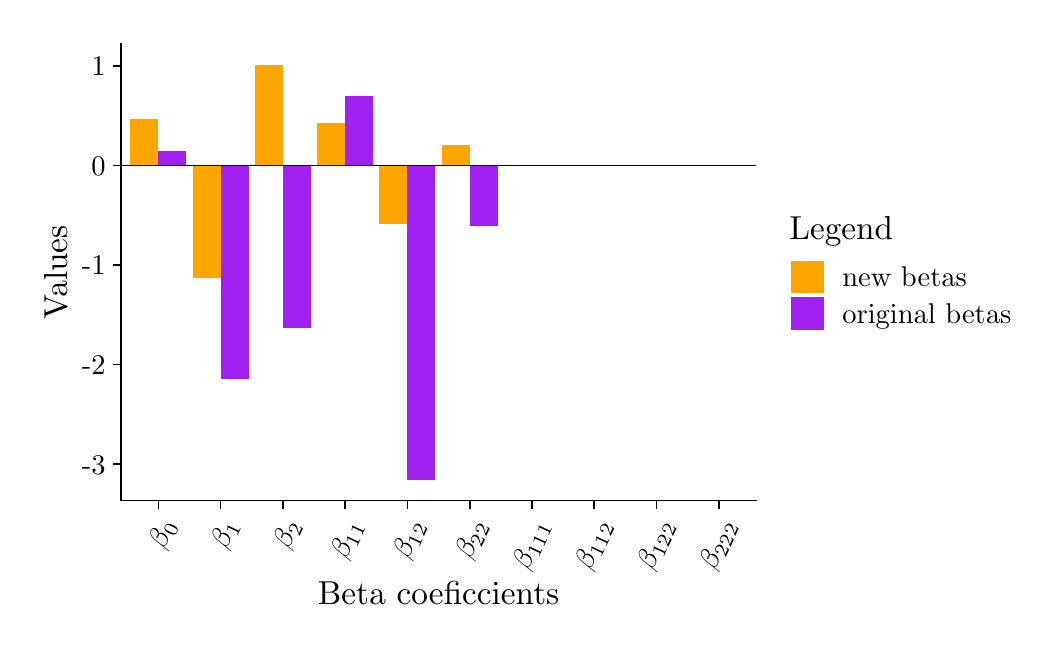
\begin{tikzpicture}[x=1pt,y=1pt]
\definecolor{fillColor}{RGB}{255,255,255}
\path[use as bounding box,fill=fillColor,fill opacity=0.00] (0,0) rectangle (361.35,216.81);
\begin{scope}
\path[clip] ( 33.74, 45.90) rectangle (263.20,210.81);
\definecolor{fillColor}{RGB}{160,32,240}

\path[fill=fillColor] ( 47.24,167.01) rectangle ( 57.36,172.20);
\definecolor{fillColor}{RGB}{255,165,0}

\path[fill=fillColor] ( 37.12,167.01) rectangle ( 47.24,183.64);
\definecolor{fillColor}{RGB}{160,32,240}

\path[fill=fillColor] ( 69.73, 89.91) rectangle ( 79.86,167.01);
\definecolor{fillColor}{RGB}{255,165,0}

\path[fill=fillColor] ( 59.61,126.50) rectangle ( 69.73,167.01);
\definecolor{fillColor}{RGB}{160,32,240}

\path[fill=fillColor] ( 92.23,108.27) rectangle (102.35,167.01);
\definecolor{fillColor}{RGB}{255,165,0}

\path[fill=fillColor] ( 82.11,167.01) rectangle ( 92.23,203.31);
\definecolor{fillColor}{RGB}{160,32,240}

\path[fill=fillColor] (114.73,167.01) rectangle (124.85,192.07);
\definecolor{fillColor}{RGB}{255,165,0}

\path[fill=fillColor] (104.60,167.01) rectangle (114.73,182.33);
\definecolor{fillColor}{RGB}{160,32,240}

\path[fill=fillColor] (137.22, 53.40) rectangle (147.34,167.01);
\definecolor{fillColor}{RGB}{255,165,0}

\path[fill=fillColor] (127.10,145.91) rectangle (137.22,167.01);
\definecolor{fillColor}{RGB}{160,32,240}

\path[fill=fillColor] (159.72,145.20) rectangle (169.84,167.01);
\definecolor{fillColor}{RGB}{255,165,0}

\path[fill=fillColor] (149.59,167.01) rectangle (159.72,174.39);
\definecolor{fillColor}{RGB}{160,32,240}

\path[fill=fillColor] (182.21,167.01) rectangle (192.34,167.01);
\definecolor{fillColor}{RGB}{255,165,0}

\path[fill=fillColor] (172.09,167.01) rectangle (182.21,167.01);
\definecolor{fillColor}{RGB}{160,32,240}

\path[fill=fillColor] (204.71,167.01) rectangle (214.83,167.01);
\definecolor{fillColor}{RGB}{255,165,0}

\path[fill=fillColor] (194.58,167.01) rectangle (204.71,167.01);
\definecolor{fillColor}{RGB}{160,32,240}

\path[fill=fillColor] (227.20,167.01) rectangle (237.33,167.01);
\definecolor{fillColor}{RGB}{255,165,0}

\path[fill=fillColor] (217.08,167.01) rectangle (227.20,167.01);
\definecolor{fillColor}{RGB}{160,32,240}

\path[fill=fillColor] (249.70,167.01) rectangle (259.82,167.01);
\definecolor{fillColor}{RGB}{255,165,0}

\path[fill=fillColor] (239.58,167.01) rectangle (249.70,167.01);
\definecolor{drawColor}{RGB}{0,0,0}

\path[draw=drawColor,line width= 0.6pt,line join=round] ( 33.74,167.01) -- (263.20,167.01);
\end{scope}
\begin{scope}
\path[clip] (  0.00,  0.00) rectangle (361.35,216.81);
\definecolor{drawColor}{RGB}{0,0,0}

\path[draw=drawColor,line width= 0.6pt,line join=round,line cap=rect] ( 33.74, 45.90) --
	( 33.74,210.81);
\end{scope}
\begin{scope}
\path[clip] (  0.00,  0.00) rectangle (361.35,216.81);
\definecolor{drawColor}{RGB}{0,0,0}

\node[text=drawColor,anchor=base east,inner sep=0pt, outer sep=0pt, scale=  1.03] at ( 28.17, 55.53) {-3};

\node[text=drawColor,anchor=base east,inner sep=0pt, outer sep=0pt, scale=  1.03] at ( 28.17, 91.51) {-2};

\node[text=drawColor,anchor=base east,inner sep=0pt, outer sep=0pt, scale=  1.03] at ( 28.17,127.49) {-1};

\node[text=drawColor,anchor=base east,inner sep=0pt, outer sep=0pt, scale=  1.03] at ( 28.17,163.47) {0};

\node[text=drawColor,anchor=base east,inner sep=0pt, outer sep=0pt, scale=  1.03] at ( 28.17,199.45) {1};
\end{scope}
\begin{scope}
\path[clip] (  0.00,  0.00) rectangle (361.35,216.81);
\definecolor{drawColor}{RGB}{0,0,0}

\path[draw=drawColor,line width= 0.6pt,line join=round] ( 30.74, 59.07) --
	( 33.74, 59.07);

\path[draw=drawColor,line width= 0.6pt,line join=round] ( 30.74, 95.05) --
	( 33.74, 95.05);

\path[draw=drawColor,line width= 0.6pt,line join=round] ( 30.74,131.03) --
	( 33.74,131.03);

\path[draw=drawColor,line width= 0.6pt,line join=round] ( 30.74,167.01) --
	( 33.74,167.01);

\path[draw=drawColor,line width= 0.6pt,line join=round] ( 30.74,202.99) --
	( 33.74,202.99);
\end{scope}
\begin{scope}
\path[clip] (  0.00,  0.00) rectangle (361.35,216.81);
\definecolor{drawColor}{RGB}{0,0,0}

\path[draw=drawColor,line width= 0.6pt,line join=round,line cap=rect] ( 33.74, 45.90) --
	(263.20, 45.90);
\end{scope}
\begin{scope}
\path[clip] (  0.00,  0.00) rectangle (361.35,216.81);
\definecolor{drawColor}{RGB}{0,0,0}

\path[draw=drawColor,line width= 0.6pt,line join=round] ( 47.24, 42.90) --
	( 47.24, 45.90);

\path[draw=drawColor,line width= 0.6pt,line join=round] ( 69.73, 42.90) --
	( 69.73, 45.90);

\path[draw=drawColor,line width= 0.6pt,line join=round] ( 92.23, 42.90) --
	( 92.23, 45.90);

\path[draw=drawColor,line width= 0.6pt,line join=round] (114.73, 42.90) --
	(114.73, 45.90);

\path[draw=drawColor,line width= 0.6pt,line join=round] (137.22, 42.90) --
	(137.22, 45.90);

\path[draw=drawColor,line width= 0.6pt,line join=round] (159.72, 42.90) --
	(159.72, 45.90);

\path[draw=drawColor,line width= 0.6pt,line join=round] (182.21, 42.90) --
	(182.21, 45.90);

\path[draw=drawColor,line width= 0.6pt,line join=round] (204.71, 42.90) --
	(204.71, 45.90);

\path[draw=drawColor,line width= 0.6pt,line join=round] (227.20, 42.90) --
	(227.20, 45.90);

\path[draw=drawColor,line width= 0.6pt,line join=round] (249.70, 42.90) --
	(249.70, 45.90);
\end{scope}
\begin{scope}
\path[clip] (  0.00,  0.00) rectangle (361.35,216.81);
\definecolor{drawColor}{RGB}{0,0,0}

\node[text=drawColor,rotate= 65.00,anchor=base east,inner sep=0pt, outer sep=0pt, scale=  1.03] at ( 53.66, 37.34) {$\beta_{0}$};

\node[text=drawColor,rotate= 65.00,anchor=base east,inner sep=0pt, outer sep=0pt, scale=  1.03] at ( 76.16, 37.34) {$\beta_{1}$};

\node[text=drawColor,rotate= 65.00,anchor=base east,inner sep=0pt, outer sep=0pt, scale=  1.03] at ( 98.65, 37.34) {$\beta_{2}$};

\node[text=drawColor,rotate= 65.00,anchor=base east,inner sep=0pt, outer sep=0pt, scale=  1.03] at (121.15, 37.34) {$\beta_{11}$};

\node[text=drawColor,rotate= 65.00,anchor=base east,inner sep=0pt, outer sep=0pt, scale=  1.03] at (143.64, 37.34) {$\beta_{12}$};

\node[text=drawColor,rotate= 65.00,anchor=base east,inner sep=0pt, outer sep=0pt, scale=  1.03] at (166.14, 37.34) {$\beta_{22}$};

\node[text=drawColor,rotate= 65.00,anchor=base east,inner sep=0pt, outer sep=0pt, scale=  1.03] at (188.64, 37.34) {$\beta_{111}$};

\node[text=drawColor,rotate= 65.00,anchor=base east,inner sep=0pt, outer sep=0pt, scale=  1.03] at (211.13, 37.34) {$\beta_{112}$};

\node[text=drawColor,rotate= 65.00,anchor=base east,inner sep=0pt, outer sep=0pt, scale=  1.03] at (233.63, 37.34) {$\beta_{122}$};

\node[text=drawColor,rotate= 65.00,anchor=base east,inner sep=0pt, outer sep=0pt, scale=  1.03] at (256.12, 37.34) {$\beta_{222}$};
\end{scope}
\begin{scope}
\path[clip] (  0.00,  0.00) rectangle (361.35,216.81);
\definecolor{drawColor}{RGB}{0,0,0}

\node[text=drawColor,anchor=base,inner sep=0pt, outer sep=0pt, scale=  1.20] at (148.47,  8.33) {Beta coeficcients};
\end{scope}
\begin{scope}
\path[clip] (  0.00,  0.00) rectangle (361.35,216.81);
\definecolor{drawColor}{RGB}{0,0,0}

\node[text=drawColor,rotate= 90.00,anchor=base,inner sep=0pt, outer sep=0pt, scale=  1.20] at ( 14.26,128.36) {Values};
\end{scope}
\begin{scope}
\path[clip] (  0.00,  0.00) rectangle (361.35,216.81);
\definecolor{drawColor}{RGB}{0,0,0}

\node[text=drawColor,anchor=base west,inner sep=0pt, outer sep=0pt, scale=  1.20] at (275.20,140.42) {Legend};
\end{scope}
\begin{scope}
\path[clip] (  0.00,  0.00) rectangle (361.35,216.81);
\definecolor{fillColor}{RGB}{255,165,0}

\path[fill=fillColor] (275.91,120.77) rectangle (287.68,132.55);
\end{scope}
\begin{scope}
\path[clip] (  0.00,  0.00) rectangle (361.35,216.81);
\definecolor{fillColor}{RGB}{160,32,240}

\path[fill=fillColor] (275.91,107.57) rectangle (287.68,119.35);
\end{scope}
\begin{scope}
\path[clip] (  0.00,  0.00) rectangle (361.35,216.81);
\definecolor{drawColor}{RGB}{0,0,0}

\node[text=drawColor,anchor=base west,inner sep=0pt, outer sep=0pt, scale=  1.03] at (294.40,123.11) {new betas};
\end{scope}
\begin{scope}
\path[clip] (  0.00,  0.00) rectangle (361.35,216.81);
\definecolor{drawColor}{RGB}{0,0,0}

\node[text=drawColor,anchor=base west,inner sep=0pt, outer sep=0pt, scale=  1.03] at (294.40,109.91) {original betas};
\end{scope}
\end{tikzpicture}
